\documentclass[aspectratio=169]{beamer}

\usepackage{beamerthemesplit}
\usepackage{amsmath}
\usepackage{amsfonts}
\usepackage{amssymb}
\usepackage{cancel}
\usepackage{bussproofs}
%% \usepackage{tkz-graph}

\makeatletter
\newcommand{\reallytiny}{\@setfontsize{\srcsize}{2pt}{2pt}}
\makeatother

\mode<presentation>
{
  \usetheme{AnnArbor}
  \usecolortheme{crane}
}

\usepackage[english]{babel}
\usepackage[latin1]{inputenc}
\usepackage{times}
\usepackage[T1]{fontenc}

\title{Temporal and Procedural Reasoning with OpenCog}

\author{Nil Geisweiller, Hedra Yusuf}

\institute[SingularityNET OpenCog Foundations]
{
  \begin{center}
    SingularityNET \& OpenCog Foundations\\
    
\includegraphics[scale=0.32]{pictures/snet_oc.png}
  \end{center}
}

\date[AGI-21]

\begin{document}

\section{Introduction}

\begin{frame}
  \maketitle
\end{frame}

\begin{frame}
  \frametitle{Why Temporal Reasoning?}

  \begin{enumerate}
    % We all know why, we live in a temporal universe, and in this
    % universe there are lags between causes and effects and we need
    % to be able to reasoning about these.
  \item Lag between cause and effect
    % And that gonna include your own thinking.  When your doing
    % meta-reasoning you need to be able to control your reasoning, at
    % some point to cut your never ending thinking loop with "Wait I
    % don't have time to think anymore", stop thinking and start
    % acting, but to think that you don't have time to think anymore,
    % you need to be able to think about time.
  \item Learn and operate in the world
  \item Meta-reasoning: {\large Think about} {\small think about}
    {\footnotesize think about} {\tiny think about ...}
  %% \item Keep thinking or act?
  \end{enumerate}
\end{frame}

\begin{frame}[fragile]
  \frametitle{PLN Recall}

  %% Given a list of predicates
\texttt{P}, \texttt{Q}, $\hdots$: $Atom^n \rightarrow \{True, False\}$
{\tiny \alert{(possibly fuzzy)}}

  \begin{columns}
    \column{1in}

\begin{semiverbatim}
  And <TV>
    P
    Q
\end{semiverbatim}

    \column{0.5in}
    $$\equiv$$

    \column{1in}
    $$\mathcal{P}(P,Q) \approx TV.strength$$

  \end{columns}

  \begin{columns}
    \column{1in}

\begin{semiverbatim}
  Not <TV>
    P
\end{semiverbatim}

    \column{0.5in}
    $$\equiv$$

    \column{1in}
    $$\mathcal{P}(P) \approx 1 - TV.strength$$

  \end{columns}

  \begin{columns}
    \column{1in}

\begin{semiverbatim}
  Implication <TV>
    P
    Q
\end{semiverbatim}

    \column{0.5in}
    $$\equiv$$

    \column{1in}
    $$\mathcal{P}(Q|P) \approx TV.strength$$

  \end{columns}

\end{frame}

\begin{frame}[fragile]

  \frametitle{PLN rules: Implication Direct Introduction}
\begin{semiverbatim}
Evaluation
  P
  Ei
...
Evaluation
  Q
  Ei
|-
Implication <TV>
  P
  Q
\end{semiverbatim}

  %% \begin{prooftree}
  %%   \AxiomC{$\texttt{Evaluation <TV> P Ei}$}
  %%   \AxiomC{$\texttt{Evaluation <TV> Q Ei}$}
  %%   \BinaryInfC{$\texttt{Implication <TV> P Q}$}
  %% \end{prooftree}


$$TV.strength = \frac{\sum_x f_\wedge(P(x).strength, Q(x).strength)}{\sum_x P(x).strength}$$
\end{frame}

\begin{frame}[fragile]

  \frametitle{PLN rules: Deduction}
\begin{semiverbatim}
Implication
  P
  Q
Implication
  Q
  R
|-
Implication <TV>
  P
  R
\end{semiverbatim}
$$TV.strength = \mathcal{P}(R|Q,P)\times\mathcal{P}(Q|P) + \mathcal{P}(R|¬Q,P)\times\mathcal{P}(¬Q|P)$$
\end{frame}

\section{Temporal Reasoning}

\begin{frame}
  \frametitle{Temporal Predicate}
\texttt{P}, \texttt{Q}, $\hdots$: $Atom^n \times Time \rightarrow \{True, False\}$
{\tiny \alert{(possibly fuzzy)}}

  \center{
    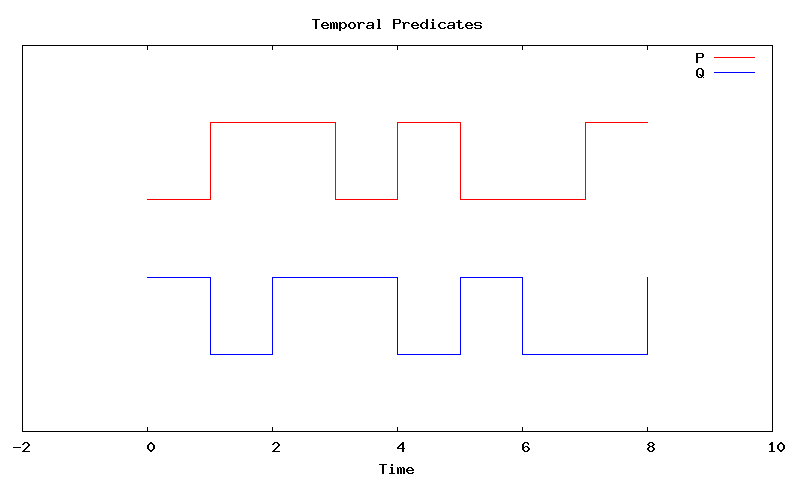
\includegraphics[scale=0.46]{pictures/tp-PQ.png}}
\end{frame}

\begin{frame}[fragile]
  \frametitle{LagLink and LeadLink}

  \begin{itemize}
  \item
  \alert{Lag}: brings \alert{past} into present
  \begin{columns}
    \column{1in}

\begin{semiverbatim}
  LagLink
    P
    T


\end{semiverbatim}

    \column{0.5in}
    $$\equiv$$

    \column{1in}
\begin{semiverbatim}
LambdaLink
  x, t
  P(x, t-T)


\end{semiverbatim}

  \end{columns}

  \item
  \alert{Lead}: brings \alert{future} into present
  \begin{columns}
    \column{1in}

\begin{semiverbatim}
  LeadLink
    P
    T
\end{semiverbatim}

    \column{0.5in}
    $$\equiv$$

    \column{1in}
\begin{semiverbatim}
LambdaLink
  x, t
  P(x, t+T)
\end{semiverbatim}

  \end{columns}
  \end{itemize}

\end{frame}

\begin{frame}
  \frametitle{Lag: example}
  \center{
    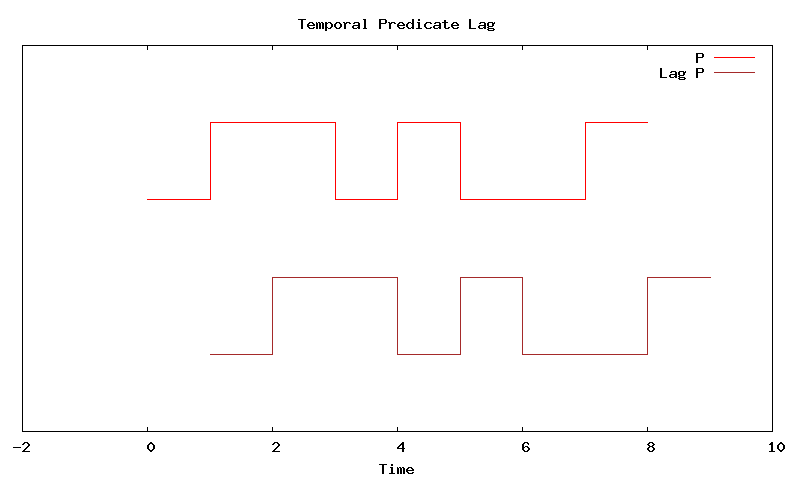
\includegraphics[scale=0.46]{pictures/tp-PLagP.png}}
\end{frame}

\begin{frame}
  \frametitle{Lead: example}
  \center{
    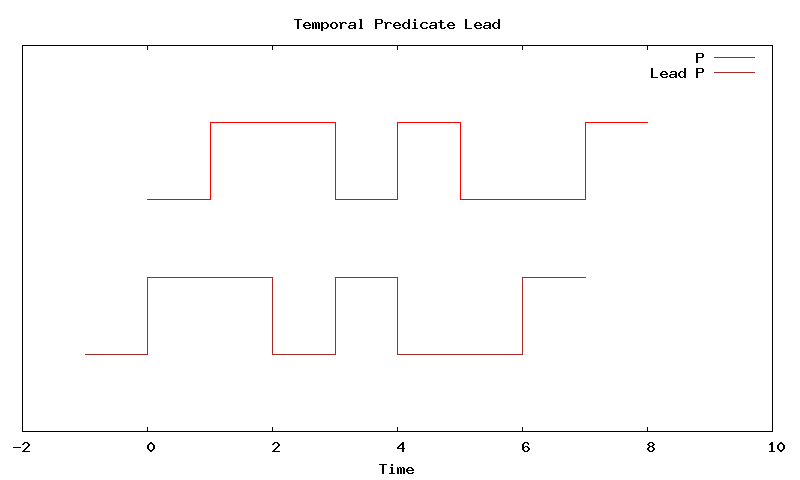
\includegraphics[scale=0.46]{pictures/tp-PLeadP.png}}
\end{frame}

\begin{frame}[fragile]
  \frametitle{SequentialAnd}

  \begin{columns}
    \column{1in}
\begin{semiverbatim}
BackSequentialAnd <TV>
  T
  P
  Q
\end{semiverbatim}

    \column{0.5in}
    $$\equiv$$

    \column{1in}
\begin{semiverbatim}
And <TV>
  Lag
    P
    T
  Q
\end{semiverbatim}

  \end{columns}

    \begin{columns}
    \column{1in}
\begin{semiverbatim}
ForeSequentialAnd <TV>
  T
  P
  Q
\end{semiverbatim}

    \column{0.5in}
    $$\equiv$$

    \column{1in}
\begin{semiverbatim}
And <TV>
  P
  Lead
    Q
    T
\end{semiverbatim}

  \end{columns}

\end{frame}


\begin{frame}[fragile]
  \frametitle{PredictiveImplication}

  \begin{columns}
    \column{1in}
\begin{semiverbatim}
BackPredictiveImplication <TV>
  T
  P
  Q
\end{semiverbatim}

    \column{0.5in}
    $$\equiv$$

    \column{1in}
\begin{semiverbatim}
Implication <TV>
  Lag
    P
    T
  Q
\end{semiverbatim}

  \end{columns}

    \begin{columns}
    \column{1in}
\begin{semiverbatim}
ForePredictiveImplication <TV>
  T
  P
  Q
\end{semiverbatim}

    \column{0.5in}
    $$\equiv$$

    \column{1in}
\begin{semiverbatim}
Implication <TV>
  P
  Lead
    Q
    T
\end{semiverbatim}

  \end{columns}

\end{frame}

\begin{frame}[fragile]
  \frametitle{PredictiveImplication}

  \begin{columns}
    \column{1in}
\begin{semiverbatim}
BackPredictiveImplication <TV>
  T
  P
  Q
\end{semiverbatim}

    \column{0.5in}
    $$\equiv$$

    \column{1in}
\begin{semiverbatim}
Implication <TV>
  Lag
    P
    T
  Q
\end{semiverbatim}

  \end{columns}

    \begin{columns}
    \column{1in}
\begin{semiverbatim}
ForePredictiveImplication <TV>
  T
  P
  Q
\end{semiverbatim}

    \column{0.5in}
    $$\equiv$$

    \column{1in}
\begin{semiverbatim}
Implication <TV>
  P
  ForeSequentialAnd
    T
    P
    Q
\end{semiverbatim}

  \end{columns}

\end{frame}

\begin{frame}[fragile]
  \frametitle{PredictiveImplication}
  \begin{columns}
    \column{2.3in}
{\small
\begin{semiverbatim}
\visible<1->{Implication <s=0.25>
  P
  Q}

\visible<2->{Implication <s=0.75>
  P
  Lead
    Q
    1}

\visible<3>{PredictiveImplication <s=0.75>
  1
  P
  Q}
\end{semiverbatim}}

  \column{3in}
  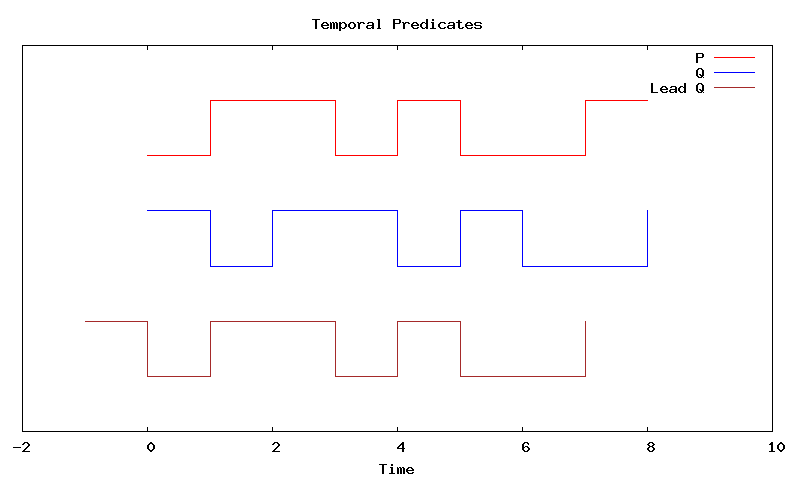
\includegraphics[scale=0.4]{pictures/tp.png}

  \end{columns}
\end{frame}

\begin{frame}[fragile]
  \frametitle{Temporal Deduction \alert{(notations)}}
  \begin{itemize}
  \item<+->
  \begin{columns}
    \column{1in}
\begin{semiverbatim}
Implication
  P
  Q
\end{semiverbatim}
    \column{0.5in}
    $$\equiv$$
    \column{1in}
    $$P \rightarrow Q$$
  \end{columns}
  \item<+->
  \begin{columns}
    \column{1in}
\begin{semiverbatim}
PredictiveImplication
  T
  P
  Q
\end{semiverbatim}
    \column{0.5in}
    $$\equiv$$
    \column{1in}
    $$P \leadsto^T Q$$
  \end{columns}

  \item<+->
  \begin{columns}
    \column{1in}
\begin{semiverbatim}
Lag
  P
  T
\end{semiverbatim}
    \column{0.5in}
    $$\equiv$$
    \column{1in}
    $$\overrightarrow{P}^T$$
  \end{columns}

  \item<+->
  \begin{columns}
    \column{1in}
\begin{semiverbatim}
Lead
  P
  T
\end{semiverbatim}
    \column{0.5in}
    $$\equiv$$
    \column{1in}
    $$\overleftarrow{P}^T$$
  \end{columns}

  \end{itemize}
\end{frame}

\begin{frame}
  \frametitle{Temporal Deduction}
  {\small
    \begin{prooftree}
      \AxiomC{$P \rightarrow Q$}
      \AxiomC{$Q \rightarrow R$}
      \AxiomC{$P$}
      \AxiomC{$Q$}
      \AxiomC{$R$}
      \RightLabel{(Deduction)}
      \QuinaryInfC{$P \rightarrow R$}
    \end{prooftree}
  }

  \pause

    {\small
    \begin{prooftree}
      \AxiomC{$P \leadsto^{T_1} Q$}
      \AxiomC{$Q \leadsto^{T_2} R$}
      \AxiomC{$P$}
      \AxiomC{$Q$}
      \AxiomC{$R$}
      \RightLabel{(Temporal Deduction?)}
      \QuinaryInfC{$P \leadsto^{T_1+T_2} R$}
    \end{prooftree}}
\end{frame}

\begin{frame}
  \frametitle{Temporal Deduction $\mapsto$ Deduction}
  {\small
    \begin{prooftree}
      \AxiomC{$P \leadsto^{T_1} Q$}
      \RightLabel{(PI2I)}
      \UnaryInfC{$P \rightarrow \overleftarrow{Q}^{T_1}$}
      \AxiomC{$Q \leadsto^{T_2} R$}
      \RightLabel{(PI2I)}
      \UnaryInfC{$Q \rightarrow \overleftarrow{R}^{T_2}$}
      \RightLabel{(TS)}
      \UnaryInfC{$\overleftarrow{Q}^{T_1} \rightarrow \overleftarrow{R}^{T_1+T_2}$}
      \AxiomC{$P$}
      \AxiomC{$Q$}
      \RightLabel{(TS)}
      \UnaryInfC{$\overleftarrow{Q}^{T_1}$}
      \AxiomC{$R$}
      \RightLabel{(TS)}
      \UnaryInfC{$\overleftarrow{R}^{T_1+T_2}$}
      \RightLabel{(Deduction)}
      \QuinaryInfC{$P \rightarrow \overleftarrow{R}^{T_1+T_2}$}
      \RightLabel{(I2PI)}
      \UnaryInfC{$P \leadsto^{T_1+T_2} R$}
    \end{prooftree}}

  \begin{itemize}
  \item TS: Temporal Shift
  \item PI2I: PredictiveImplication to Implication
  \item I2PI: Implication to PredictiveImplication
  \end{itemize}
\end{frame}

\section{Procedural Reasoning}

\begin{frame}[fragile]
  \frametitle{Procedural Reasoning (notations)}
  \begin{itemize}
  \item<+->
  \begin{columns}
    \column{1in}
\begin{semiverbatim}
SequentialAnd
  T
  P
  Q
\end{semiverbatim}
    \column{0.5in}
    $$\equiv$$
    \column{1in}
    $$P \prec^T Q$$
  \end{columns}

%%   \item
%%   \begin{columns}
%%     \column{1in}
%% \begin{semiverbatim}
%% Execution
%%   A
%%   arguments
%%   Success
%% \end{semiverbatim}
%%     \column{0.5in}
%%     $$\equiv$$
%%     \column{1in}
%%     $$!A(<arguments>)$$
%%   \end{columns}
  \item<+->
  \begin{columns}
    \column{1in}
\begin{semiverbatim}
Lambda
  T
  AtTime
    Execution
      A
    T
\end{semiverbatim}
    \column{0.5in}
    $$\equiv$$
    \column{1in}
    $$\widehat{A}$$
  \end{columns}
  \end{itemize}
\end{frame}

\begin{frame}
  \frametitle{Cognitive Schematics}

  \begin{itemize}
  \item<+-> Monoaction plan
    $$C \wedge \widehat{A} \leadsto^{T} G$$
  \item<+-> Diaction plan
    $$\left( (C \wedge \widehat{A_1} ) \prec^{T_1} \widehat{A_2} \right) \leadsto^{T_1+T_2} G$$
  \item<+-> Polyaction plan
    $$\left( \left( \left( Inside \wedge \widehat{WalkToDoor}\right) \prec^{2}
    \widehat{OpenDoor}\right) \prec^{3} \widehat{StepOut}\right) \leadsto^{6} Outside$$
  \end{itemize}

\end{frame}

\begin{frame}
  \frametitle{Temporal Deduction for Procedural Reasoning}
  {\tiny
    \begin{prooftree}
      \AxiomC{$P \wedge \widehat{A} \leadsto^{T_1} Q$}
      \RightLabel{(PI2I)}
      \UnaryInfC{$P \wedge \widehat{A} \rightarrow
        \overleftarrow{Q}^{T_1}$}
      \AxiomC{$\widehat{B}$}
      \RightLabel{(TS)}
      \UnaryInfC{$\overleftarrow{\widehat{B}}^{T_1}$}
      \RightLabel{(CI)}
      \BinaryInfC{$P \wedge \widehat{A} \wedge
        \overleftarrow{\widehat{B}}^{T_1} \rightarrow
        \overleftarrow{Q}^{T_1} \wedge \overleftarrow{\widehat{B}}^{T_1}$}
      \AxiomC{$Q \wedge \widehat{B} \leadsto^{T_2} R$}
      \RightLabel{(PI2I)}
      \UnaryInfC{$Q \wedge \widehat{B} \rightarrow \overleftarrow{R}^{T_2}$}
      \RightLabel{(TS)}
      \UnaryInfC{$\overleftarrow{Q}^{T_1} \wedge
        \overleftarrow{\widehat{B}}^{T_1} \rightarrow
        \overleftarrow{R}^{T_1+T_2}$}
      %% \AxiomC{$P \wedge \widehat{A}$}
      %% \AxiomC{$\overleftarrow{\widehat{B}}^{T_1}$}
      %% \RightLabel{(CI)}
      \AxiomC{$P \wedge \widehat{A} \wedge \overleftarrow{\widehat{B}}^{T_1}$}
      \AxiomC{$Q \wedge \widehat{B}$}
      \RightLabel{(TS)}
      \UnaryInfC{$\overleftarrow{Q}^{T_1} \wedge \overleftarrow{\widehat{B}}^{T_1}$}
      \AxiomC{$R$}
      \RightLabel{(TS)}
      \UnaryInfC{$\overleftarrow{R}^{T_1+T_2}$}
      \RightLabel{(D)}
      \QuinaryInfC{$P \wedge \widehat{A} \wedge \overleftarrow{\widehat{B}}^{T_1} \rightarrow \overleftarrow{R}^{T_1+T_2}$}
      \RightLabel{(I2PI)}
      \UnaryInfC{$\left( (P \wedge \widehat{A}) \prec^{T_1}
        \widehat{B} \right) \leadsto^{T_1+T_2} R$}
    \end{prooftree}}

  \begin{itemize}
  \item D: Deduction
  \item CI: Conjunction Introduction
  \item TS: Temporal Shift
  \item PI2I: PredictiveImplication to Implication
  \item I2PI: Implication to PredictiveImplication
  \end{itemize}

\end{frame}

\begin{frame}
  \frametitle{Procedural Reasoning Example}
  $$\left( \left( Inside \wedge \widehat{WalkToDoor}\right)
  \prec^{2} \widehat{OpenDoor}\right) \leadsto^{3} OpenDoorStep$$
  $$OpenDoorStep \wedge \widehat{StepOut} \leadsto^{1} Outside$$
  $$\vdash$$
  $$\left( \left( \left( Inside \wedge \widehat{WalkToDoor}\right)
  \prec^{2} \widehat{OpenDoor}\right) \prec^{3} \widehat{StepOut}\right) \leadsto^{6} Outside$$
\end{frame}

\section{Conclusion}

\begin{frame}
  \frametitle{Temporal and Procedural Reasoning: next steps}
  \begin{itemize}
  \item<+-> More rules
    \begin{itemize}
    \item Temporal Abduction
    \item $\dots$
    \end{itemize}
  %% \item<+-> Temporal Pattern Miner
  \item<+-> Distributional Time
    \begin{itemize}
    \item Temporal Interval
      $$(((Inside \wedge \widehat{WalkToDoor}) \prec^{[1,2]}
    \widehat{OpenDoor}) \prec^{[1.5,3]} \widehat{StepOut}) \leadsto^{[1.6,4]}
    Outside$$
  \item Temporal Truth Value
      $$(((Inside \wedge \widehat{WalkToDoor}) \prec
    \widehat{OpenDoor}) \prec \widehat{StepOut}) \leadsto Outside$$
    \end{itemize}
  \item<+-> Behavior Tree
    {\small
      $$(((Inside \wedge \widehat{WalkToDoor}) \prec
    (Locked\ ?\ \widehat{SmashDoor}\ :\ \widehat{OpenDoor})) \prec \widehat{StepOut}) \leadsto Outside$$}
  \item<+-> Dependent Truth Value (or Density Truth Value)
  \end{itemize}
\end{frame}

\begin{frame}
  \frametitle{Conclusion}
  \begin{center} Demo Time \end{center}
\end{frame}
\end{document}
